\newpage
\section{Exercise Block 1}

\subsection{Exclusive OR (15min)}\label{subsec:ex-1}
\textbf{Construct an XOR gate using only the giant NAND gates.}

 XOR stands for exclusive OR. As the name suggest, it is very similar to the OR gate, except that it does not yield one when both inputs are one. In different words this means that the XOR is true whenever the two inputs are not equal. Follow the steps below to construct the XOR circuit.
\begin{enumerate}
	\item Write down the truth table.
	\item\label{it:1} Construct the disjunctive normal form from your truth table.
	\item Draw the circuit according to step \ref{it:1}.
	\item Transform the circuit in such a way that it only uses NAND Gates.
	\item Build the XOR you have drawn with the giant NAND gates.
	\item How many NAND gates do you need? See if you can loose one or two gates.
\end{enumerate}

\subsection{XOR to the Next (15min)}
\textbf{Construct the same XOR gate as in exercise \ref{subsec:ex-1} but this time with the breadboard using the tiny gates.}


\section{Excercise Block 2a}

\subsection{Half-Adder (30min)}
\subsubsection{Part 1}
A half-adder takes two bits $a$ and $b$ and adds them. It is called half-adder because two of them are needed in order to construct an adder which is able to add several bits. We will see later why this is the case.

Let's first look at the addition of two decimal digits. 

\begin{figure}[h]
	\centering		  
	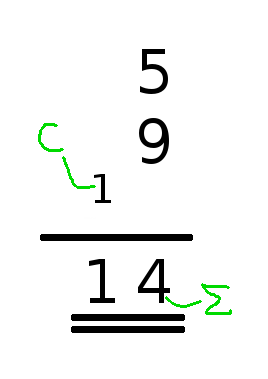
\includegraphics[scale=0.3]{decimal_addition.png}
	\caption{Decimal addition.}
	\label{fig:decimal_addition}
\end{figure}
We see that we need two things:
\begin{itemize}
	\item We need to know in which number the combination of 5 and 9 results. Namely 4.
	\item We need to carry a digit 1 because $5+9$ exceeds 10.
\end{itemize}

For binary digits (bits) we can do the same thing. Let's assume the following case. We have two 1 digit binary numbers. We call the single bit of the first number $a$ and the single bit of the second number $b$.
\begin{itemize}
	\item Write down all possible combinations of $a$ and $b$ in table \ref{tab:half-adder-truth-table}.
	\item Think about the output of each combination of $a$ and $b$ and write it into table \ref{tab:half-adder-truth-table} in the column $out$. Which logical circuit does this resemble?
	\item Similar to the decimal case, we need to sometimes carry a bit. Write the value of the carry bit $c$ into table \ref{tab:half-adder-truth-table}. Now look at the columns $a$, $b$ and $c$. Which logical circuit does this resemble?
	
\end{itemize}
\begin{table}[H]
	\centering
	\begin{tabular}{|c|c||c|c|}
		\hline
		$a$ & $b$ & $out$   & $c$ \\ \hline
		&     &           &       \\ \hline
		&     &           &       \\ \hline
		&     &           &       \\ \hline
		&     &           &       \\ \hline
	\end{tabular}
	\caption{Truth table for the Half Adder.}
	\label{tab:half-adder-truth-table}
\end{table}

\subsection{Full-Adder (30min)}

\section{Exercise Block 2b}
\subsection{D FlipFlop}
\subsection{D Master Slave}

\newpage